\newcommand{\chapter}[2][]{
	\newcommand{\chapname}{#2}
	\begin{flushleft}
		\begin{minipage}[t]{\linewidth}
			
\includegraphics[height=1cm]{hdht-logo.png}
			\hspace{0pt}	
			\sffamily\bfseries\large Bài  17.
			\begin{flushleft}
				\LARGE\bfseries #1
			\end{flushleft}
		\end{minipage}
	\end{flushleft}
	\vspace{1cm}
	\normalfont\normalsize
}
\chapter[Một số loại lực thường gặp trong thực tiễn: \\trọng lực, lực căng dây, lực đàn hồi]{Một số loại lực thường gặp trong thực tiễn:\\ Trọng lực, lực căng dây, lực đàn hồi}
\section{Lý thuyết}

\subsection{Trọng lực - Lực hấp dẫn}
\vspace{-0.5cm}
\subsubsection{Lực hấp dẫn}
Mọi vật trong vũ trụ đều hút nhau với một lực, gọi là lực hấp dẫn.

 Đặc điểm của lực hấp dẫn:	
\begin{itemize}
	\item Luôn là lực hút;
	\item Là lực không tiếp xúc (tác dụng từ xa).
\end{itemize}

\subsubsection{Định luật vạn vật hấp dẫn} 
	\begin{center}
	\begin{tikzpicture}
		\coordinate (A1) at (0,0);
		\coordinate (A2) at ($(A1)+(1.5cm,0)$);
		\coordinate (B1) at ($(A1)+(6cm,0)$);
		\coordinate (B2) at ($(B1)-(1.5cm,0)$);
		\shade[ball color=green] (A1) circle (0.75cm); 
		\shade[ball color=purple] (B1) circle (0.5cm);
		\draw[dashed] (A1) -- (B1);
		\draw[->,very thick] (A1)--(A2) node[near end,above right]{$\vec{F}_{12}$};
		\draw[->,very thick] (B1)--(B2) node[near end,above left]{$\vec{F}_{21}$};
		\coordinate (Ad) at ($(A1)-(0,2cm)$);
		\coordinate (Bd) at ($(B1)-(0,2cm)$);
		\draw[dotted] (A1) -- (Ad);
		\draw[dotted] (B1) -- (Bd);
		\draw[<->] (Ad) --(Bd);
		\node[below=1cm, fill=pagecol] at (A1) {$m_1$};
		\node[below=0.75cm, fill=pagecol] at (B1) {$m_2$};
		\node[fill=pagecol] at ($(Ad)!0.5!(Bd)$) {$r$};
	\end{tikzpicture}
\end{center}
%\begin{center}
%	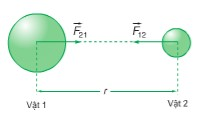
\includegraphics[scale=1.3]{../figs/VN10-PH-13-L-010-1-V2-01.jpg}
%\end{center}
Lực hấp dẫn giữa hai chất điểm bất kì tỉ lệ thuận với tích hai khối lượng của chúng và tỉ lệ nghịch với bình phương khoảng cách giữa chúng.
\begin{equation*}
	F_{\text {hd}} = G \dfrac {m_1 m_2 }{r^2},
\end{equation*}
trong đó:
\begin{itemize}
	\item $G$ là hằng số hấp dẫn, trong hệ SI có giá trị $G=\SI{6.67e-11}{\newton \meter ^2/\kilogram ^2}$;
	\item $m_1$, $m_2$ là khối lượng của hai vật;
	\item $r$ là khoảng cách giữa hai vật.
\end{itemize}

\subsubsection{Trọng lực }

Trọng lực là lực của Trái đất tác dụng vào vật gây ra cho chúng gia tốc rơi tự do. Trọng lực kí hiệu là $\vec P.$

\begin{equation*}
	P=F_{\text{hd}}=G \dfrac {mM}{(R+h)^2},
\end{equation*}
trong đó:
\begin{itemize}
	\item $m$ là khối lượng của vật ($\SI{}{\kilogram}$);
	\item $M$ là khối lượng Trái đất ($M \approx \SI{6e24}{\kilogram}$);
	\item $R$ là bán kính Trái đất ($R \approx \SI{6400e3}{\meter}$);
	\item $h$ là  độ cao của vật so với mặt đất ($\SI{}{\meter}$).
\end{itemize}

Gia tốc rơi tự do:
\begin{equation*}
	g=G \dfrac {M}{(R+h)^2}.
\end{equation*}
\begin{center}
	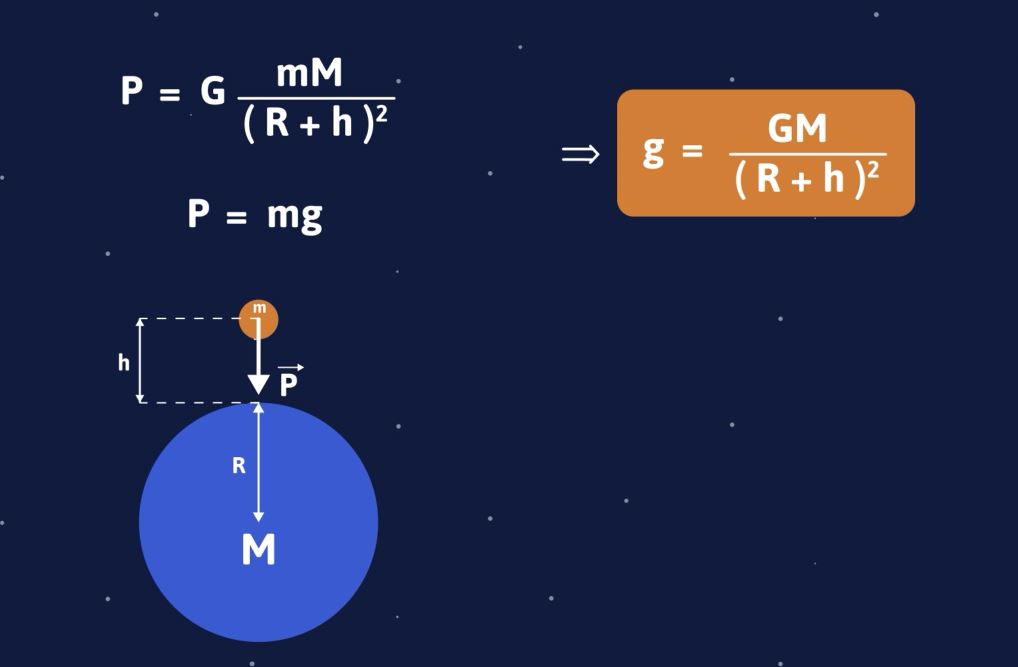
\includegraphics[scale=0.4]{../figs/VN10-PH-13-A-004-1-V2-01.jpg}
\end{center}

Ở gần Trái đất, trọng lực có phương thẳng đứng, có chiều từ trên xuống. % và đặt vào một điểm đặc biệt của mỗi vật, gọi là trọng tâm của vật.
%Hưng comment: chương này đang là động lực học chất điểm, không cần đưa vào khái niệm trọng tâm vì vật chỉ là chất điểm, không có kịch thước. 
Công thức tính trọng lực: 
\begin{equation*}
	\vec P=m\vec g.
\end{equation*}

\subsubsection{Trọng lượng}
%Độ lớn của trọng lực tác dụng lên một vật gọi là trọng lượng của vật, kí hiệu là $P$.
%Hưng comment: định nghĩa sai nghiêm trọng, sửa lại như bên dưới. 

Khi vật đặt trong trọng trường và ở trạng thái cân bằng nhờ một dây treo hay giá đỡ, thì độ lớn của lực căng dây hoặc lực ép của vật lên giá đỡ gọi là trọng lượng của vật.  

\luuy{Không nên nhầm lẫn rằng trọng lượng là độ lớn của trọng lực. 
	
	Ví dụ, phi hành gia trên các trạm vũ trụ vẫn chịu tác dụng của trọng lực $P=mg$. Tuy nhiên nếu đặt một cái cân dưới chân phi hành gia thì cân chỉ số 0, vì trọng lực đã cân bằng với lực quán tính ly tâm (do trạm vũ trụ quay quanh Trái đất), nên phi hành gia không tạo được sức ép vào mặt cân. Ta nói phi hành gia ở trạng thái không trọng lượng (chứ không phải không trọng lực). }
\subsection{Lực căng dây}
\begin{minipage}[l]{0.6\textwidth}
	Khi kéo căng một sợi dây thì trong sợi dây xuất hiện lực căng chống lại xu hướng bị kéo dãn, gọi là lực căng dây.
	
%	Nếu dây đứng yên, độ lớn lực căng dây là như nhau tại tất cả các điểm trên dây.
	
%	Khi dây chuyển động, độ lớn lực căng dây tại mọi điểm trên dây vẫn như nhau nếu dây mảnh và khối lượng không đáng kể.
%Hưng comment: độ lớn lực căng dây như nhau tại mọi điểm nếu dây không co giãn (vd dây thun) và khối lượng không đáng kể, không phụ thuộc vào việc dây có chuyển động hay không. 	
	
	Đối với dây không co giãn và khối lượng không đáng kể, độ lớn lực căng dây là như nhau tại mọi điểm trên dây. 
	
\end{minipage}
\begin{minipage}[r]{0.4\textwidth}
	\begin{center}
		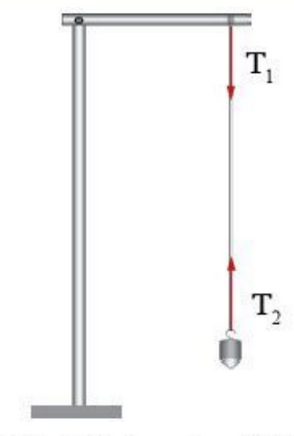
\includegraphics[scale=0.5]{../figs/G10-18-1}
	\end{center}
\end{minipage}

\subsection{Lực đàn hồi}
\subsubsection{Khái niệm lực đàn hồi}
	Lực đàn hồi là lực sinh ra khi vật đàn hồi bị biến dạng. Lực đàn hồi có xu hướng chống lại nguyên nhân gây ra biến dạng (tức là làm cho vật lấy lại hình dạng và kích thước ban đầu).
\subsubsection{Giới hạn đàn hồi}
	Khi độ biến dạng lớn vượt quá một giới hạn nào đó thì  vật bị biến dạng sẽ không thể trở về được hình dạng ban đầu. Ta gọi giới hạn này là giới hạn đàn hồi. 		

\subsubsection{Lực đàn hồi của lò xo}
	Khi lò xo bị biến dạng trong giới hạn đàn hồi, trong lò xo xuất hiện lực đàn hồi có chiều chống lại chiều biến dạng của lò xo, độ lớn tuân theo định luật Hooke: 
		\begin{equation}
			F_\text{đh}= k \cdot |\Delta l|.
		\end{equation}
	
	trong đó:
		\begin{itemize}
			\item $k$ là độ cứng của lò xo (N/m).
			\item $|\Delta l|=|l-l_0|$ là độ biến dạng của lò xo (m), với $l$ và $l_0$ là độ dài lò xo khi bị biến dạng và khi không bị biến dạng. 
		\end{itemize}
	Cũng giống lực căng dây, lực đàn hồi của lò xo có độ lớn như nhau tại mọi điểm của lò xò. 
\section{Mục tiêu bài học - Ví dụ minh họa}
\begin{dang}{Ghi nhớ định luật vạn vật hấp dẫn. \\Nhận biết được đặc điểm của lực hấp dẫn}
	\viduii{1}{Lực hấp dẫn do một hòn đá ở trên mặt đất tác dụng vào Trái đất thì có độ lớn
		\begin{mcq}(2)
			\item lớn hơn trọng lực của hòn đá.
			\item nhỏ hơn trọng lực của hòn đá.
			\item bằng trọng lưc của hòn đá. 
			\item bằng 0.
		\end{mcq}
	}
	{	\begin{center}
			\textbf{Hướng dẫn giải}
		\end{center}
		
		Trọng lực là trường hợp riêng của lực hấp dẫn
		
		\textbf{Đáp án: C.}
	}
	\viduii{1}{Chọn phát biểu sai về lực hấp dẫn giữa hai vật?
		\begin{mcq}
			\item Lực hấp dẫn tăng 4 lần khi khoảng cách giảm đi một nửa .
			\item Lực hấp dẫn không đổi khi khối lượng một vật tăng gấp đôi còn khối lượng vật kia giảm còn một nửa.
			\item Rất hiếm khi lực hấp dẫn là lực đẩy.
			\item Hằng số hấp dẫn có giá trị như nhau ở cả trên mặt Trái đất và trên Mặt trăng.
		\end{mcq}
		
	}
	{	\begin{center}
			\textbf{Hướng dẫn giải}
		\end{center}
		
		Lực hấp dẫn luôn là lực hút.
		
		\textbf{Đáp án: C.}
	}
\end{dang}

\begin{dang}{Tính lực hấp dẫn và các đại lượng trong công thức của định luật vạn vật hấp dẫn}
	\viduii{3}{Cho biết khoảng cách giữa tâm Mặt trăng và tâm Trái đất là $\SI{38e7}{\meter}$; khối lượng Mặt trăng và Trái đất tương ứng là $\SI{7.37e22}{\kilogram}$ và $\SI{6e24}{\kilogram}$; hằng số hấp dẫn $G = \SI{6.67e-11}{\newton \meter ^2 / \kilogram ^2}$. Lực hấp dẫn giữa Trái đất và Mặt trăng có độ lớn là
		\begin{mcq}(2)
			\item $\SI{0.204e21}{\newton}$.
			\item $\SI{2.04e21}{\newton}$.
			\item $\SI{22e2}{\newton}$.
			\item $\SI{2e27}{\newton}$.
		\end{mcq}
	}
	{	\begin{center}
			\textbf{Hướng dẫn giải}
		\end{center}
		
		Áp dụng công thức lực hấp dẫn giữa Trái đất và Mặt trăng
		$$	F_{\text{hd}}=G\dfrac {m_1 m_2}{r^2} = \SI{0.204e21}{\newton}.$$
		
		\textbf{Đáp án: A.}
		
	}
	\viduii{3}{Hai quả cầu giống nhau được đặt sao cho hai tâm cách nhau khoảng $r$ thì lực hấp dẫn giữa chúng là $F$. Nếu thay một trong hai khối cầu trên bằng một khối cầu đồng chất khác nhưng có bán kính lớn gấp hai, vẫn giữ nguyên khoảng cách giữa hai tâm (hai khối cầu không chạm nhau) thì lực hấp dẫn giữa chúng lúc này là
		\begin{mcq}(4)
			\item $2F$.
			\item $4F$.
			\item $8F$.
			\item $16F$.
		\end{mcq}
		
	}
	{	\begin{center}
			\textbf{Hướng dẫn giải}
		\end{center}
		
		Gọi quả cầu 2 là quả cầu có bán kính tăng gấp đôi. Bán kính của quả cầu 2 lúc sau
		$$r_2 ' = 2 r_2.$$
		
		Nếu $D$ là khối lượng riêng của quả cầu thì khối lượng của quả cầu 2 lúc sau sẽ là 
		$$m_2 ' = D V_2 ' = D \dfrac{4}{3}\pi {r'}_2^3= D \dfrac {4}{3} \pi (2r_2) ^3 = 8 D \dfrac {4}{3}\pi r_2 ^3 = 8 D V_2 = 8 m_2. $$
		
		Lực hấp dẫn giữa hai quả cầu lúc sau
		$$F_\text{hd}' = G \dfrac{m_1 m_2 '}{r^2} = 8 G \dfrac {m_1 m_2}{r^2} = 8F.$$
		
		\textbf{Đáp án: C.}
	}
\end{dang}
\begin{dang}{Tính gia tốc rơi tự do và  trọng lượng vật trong các điều kiện khác nhau}
	\viduii{3}{Ở độ cao nào so với mặt đất thì gia tốc rơi tự do bằng một nửa gia tốc rơi tự do ở mặt đất? Cho bán kính Trái Đất là $R=\SI{6400}{\kilo \meter}$.
	}
	{	\begin{center}
			\textbf{Hướng dẫn giải}
		\end{center}
		
		Gia tốc rơi tự do ở mặt đất:
		$$g_0 = G \dfrac {M}{R^2}.$$
		
		Gia tốc rơi tự do ở độ cao $h$:
		$$g=G \dfrac {M}{(R+h)^2}.$$
		
		Gia tốc rơi tự do ở độ cao $h$ bằng một nửa gia tốc rơi tự do ở mặt đất, nên
		$$g=\dfrac{g_0}{2} \Rightarrow G \dfrac {M}{(R+h)^2} = G \dfrac {M}{2R^2} \Rightarrow (R+h)^2 = 2 R^2 \Rightarrow h=\SI{2650}{\kilo \meter}.$$
		
		Vậy ở độ cao $h=\SI{2650}{\kilo \meter}$ so với mặt đất thì gia tốc rơi tự do bằng một nửa so với gia tốc rơi tự do ở mặt đất.
		
	}
	\viduii{3}{Tính độ cao mà ở đó gia tốc rơi tự do là 9,6 m/s$^2$. Biết bán kính Trái Đất là 6400 km và gia tốc rơi tự do ở sát mặt đất là 9,8 m/s$^2$.
		
	}
	{	\begin{center}
			\textbf{Hướng dẫn giải}
		\end{center}
		
		Gia tốc rơi tự do ở độ cao $h$ 
			\begin{equation*}
				g = \dfrac{GM}{(R+h)^2} = \text{9,6}\ \text{m/s}^2.
			\end{equation*}
		Gia tốc rơi tự do ở sát mặt đất 
			\begin{equation*}
				g_0 = \dfrac{GM}{R^2} = \text{9,8}\ \text{m/s}^2.
			\end{equation*}
		Suy ra 
			\begin{equation*}
				\dfrac{g}{g_0}= \left(\dfrac{R}{R+h}\right)^2 =\text{0,98}\Rightarrow h = \dfrac{R(1- \sqrt{\text{0,98}})}{\sqrt {\text{0,98}}} = 65\ \text{km}.
			\end{equation*}
		
	}
	
	\viduii{3}{Tính gia tốc rơi tự do và trọng lực của một vật có khối lượng $m = 50\ \text{kg}$ ở độ cao $\dfrac{7}{9}$ bán kính Trái Đất. Biết gia tốc rơi tự do ở sát mặt đất là 10 m/s$^2$ và bán kính Trái Đất là 6400 km. Ở độ cao bằng $\dfrac{7}{9}$ bán kính Trái Đất nếu có một vệ tinh nhân tạo chuyển động tròn đều xung quanh Trái Đất thì vệ tinh bay với tốc độ dài bằng bao nhiêu và cần thời gian bao lâu để bay hết một vòng?
	}
	{	\begin{center}
			\textbf{Hướng dẫn giải}
		\end{center}
		
		Gia tốc rơi tự do ở độ cao $h$ 
		\begin{equation*}
			g = \dfrac{GM}{(R+h)^2}.
		\end{equation*}
		Gia tốc rơi tự do ở sát mặt đất 
		\begin{equation*}
			g_0 = \dfrac{GM}{R^2}.
		\end{equation*}
		Ta lập tỉ số  
		\begin{align*}
			\dfrac{g}{g_0}&= \left(\dfrac{R}{R+h}\right)^2 =\left(\dfrac{R}{R+\dfrac{7}{9}R}\right)^2=\left(\dfrac{9}{16}\right)^{2}\\
			\Rightarrow\quad g&= \left(\dfrac{9}{16}\right)^2g_0=\left(\dfrac{9}{16}\right)^2\times\SI{9.81}{\meter/\second^{2}}\approx \SI{3.1}{\meter/\second^{2}}.
		\end{align*}
		Trọng lực  của vật ở độ cao đó
			\begin{equation*}
				P = mg= 160\ \text{N}.
			\end{equation*}
		Trọng lực đóng vai trò lực hướng tâm trong chuyển động quay đều của vệ tinh quanh Trái đất, do đó 
			\begin{equation*}
				F_{\text{ht}} =m\dfrac{v^2}{r} = mg \Rightarrow v=\sqrt{rg}=\sqrt{\left(R+\dfrac{7}{9}R\right) g} = \dfrac{4}{3} \sqrt{Rg} \approx \SI{6000}{\meter/\second}.
			\end{equation*}
		Chu kỳ quay của vệ tinh
			\begin{equation*}
				T =\dfrac{2\pi}{\omega}= \dfrac{2\pi r}{v} = \dfrac{2\pi \left(R+\dfrac{7}{9}R\right)}{v}\approx\SI{11900}{\second}\approx\SI{3}{\hour}\ \SI{18}{\minute}. 
			\end{equation*}
		
	}
\end{dang}
\begin{dang}{Nhận biết đặc điểm của lực đàn hồi \\Ghi nhớ định luật Húc}
	\viduii{1}{Lực đàn hồi xuất hiện tỉ lệ với độ biến dạng khi 
		\begin{mcq}
			\item một vật bị biến dạng dẻo.
			\item một vật biến dạng đàn hồi.
			\item một vật bị biến dạng.	
			\item ta ấn ngón tay vào một viên đất nặn.
		\end{mcq}
	}
	{	\begin{center}
			\textbf{Hướng dẫn giải}
		\end{center}
		
		Lực đàn hồi xuất hiện tỉ lệ với độ biến dạng khi một vật biến dạng đàn hồi.
		
		\textbf{Đáp án: B}.
	}
	\viduii{1}{Điều nào sau đây là sai?
		\begin{mcq}
			\item Độ cứng của lò xo cũng được gọi là hệ số đàn hồi của lò xo.
			\item Lò xo có độ cứng càng nhỏ càng khó biến dạng.
			\item Độ cứng cho biết sự phụ thuộc tỉ lệ của độ biến dạng của lò xo vào lực gây ra sự biến dạng đó.
			\item Độ cứng phụ thuộc hình dạng, kích thước lò xo và chất liệu làm lò xo.
		\end{mcq}
	}
	{	\begin{center}
			\textbf{Hướng dẫn giải}
		\end{center}
		
		Lò xo có độ cứng càng lớn càng khó biến dạng.
		
		\textbf{Đáp án: B}.
	}
\end{dang}
\begin{dang}{Tính độ biến dạng của lò xo \\và các đại lượng theo định luật Hooke}
	\viduii{3}{Một lò xo có chiều dài tự nhiên là $\SI{30}{cm}$, khi bị nén lò xo dài $\SI{24}{cm}$ và lực đàn hồi của nó bằng $\SI{5}{N}$. Hỏi khi lực đàn hồi bị nén bằng $\SI{10}{N}$ thì chiều dài của nó bằng bao nhiêu?
	}
	{	\begin{center}
			\textbf{Hướng dẫn giải}
		\end{center}
		
		Độ biến dạng của lò xo khi bị nén còn $\SI{24}{\centi\meter}$ là
			\begin{equation*}
				\Delta l = l_0 - l = \SI{6}{cm}.
			\end{equation*}
		Độ cứng của lò xo được suy ra từ định luật Hooke
			\begin{equation*}
				F=k\Delta l \quad\Rightarrow\quad k= \dfrac{F}{\Delta l} = \dfrac{250}{3}\ \text{N/m}.
			\end{equation*}
		Khi lực đàn hồi của lò xo bị nén bằng lực 10 N thì độ biến dạng tương ứng là 
			\begin{equation*}
				\Delta l' =\dfrac{F'}{k} = \SI{0,12}{cm}.
			\end{equation*}
		Chiều dài của lò xo lúc này
			\begin{equation*}
				l=l_0 -\Delta l = \SI{18}{cm}.
			\end{equation*} 
		
	}
	\viduii{2}{Một quả cân có khối lượng $m = \SI{100}{g}$ treo vào đầu dưới của một lò xo nhẹ, đầu kia của lò xo gắn trên giá treo. Cho $g= \SI{10}{m/s^2}$. Khi vật cân bằng thì lực của lò xo tác dụng lên vật là bao nhiêu?  Lò xo bị nén hay dãn?
	}
	{	\begin{center}
			\textbf{Hướng dẫn giải}
		\end{center}
		
		Vật chịu tác dụng của trọng lực $\vec{P}$ và lực đàn hồi $\vec{F}_{\text{đh}}$. 	Khi vật nằm cân bằng thì hai lực này phải trực đối nhau, nghĩa là $\vec{F}_{\text{đh}}$ hướng lên, tức là lò xo bị kéo dãn xuống, độ lớn lực đàn hồi bằng đúng trọng lực 
			\begin{equation*}
				F_{\text{đh}} = P = mg =\SI{1}{N}.
			\end{equation*}
		
	}
\end{dang}

%1. hình 1 mờ, cần vẽ lại hoặc chụp lại sắc nét hơn.
%2. định nghĩa cũ của trọng lượng:
%	"Độ lớn của trọng lực tác dụng lên một vật gọi là trọng lượng của vật, kí hiệu là $P$. "
%	là định nghĩa sai nghiêm trọng 

